\documentclass[10pt]{beamer}
\usepackage{../../../resources/themes/algolymp-dense}
\usepackage{booktabs}
\usepackage{amssymb}
\usepackage{tikz}

\title{Arbore Indexat Binar}
\subtitle{Variante și implementări}
\author{Andrei Mihai Ciobanu}
\institute{Algolymp Summer School}
\date{}
\titlegraphic{\includegraphics[width=3cm]{../../../resources/algolymp-logo.png}}
\setbeamertemplate{frame footer}{Algolymp \textemdash{} Lot Juniori}

% ================================================================
\begin{document}

\begin{frame}
  \titlepage
\end{frame}

\begin{frame}{Cuprins}
  \tableofcontents[hideallsubsections]
\end{frame}

% ================================================================
\section{AIB Clasic \textemdash{} Point add, range sum}

\begin{frame}{Problema de bază}
  \begin{block}{Problemă}
    Dat un șir $a_1, \ldots, a_n$. Se efectuează $q$ operații:
    \begin{itemize}\itemsep0pt
      \item \textbf{Point add:} adaugă $x$ la $a_i$
      \item \textbf{Range sum:} calculează $\sum_{j=l}^{r} a_j$
    \end{itemize}
  \end{block}
  \smallskip
  \textbf{Abordări naive:}
  \begin{center}
  \begin{tabular}{lcc}
    \toprule
    Metodă & Update & Query \\
    \midrule
    Array simplu & $O(1)$ & $O(n)$ \\
    Sume parțiale & $O(n)$ (recompilare) & $O(1)$ \\
    \textbf{AIB} & $\mathbf{O(\log n)}$ & $\mathbf{O(\log n)}$ \\
    \bottomrule
  \end{tabular}
  \end{center}
  \smallskip
  Soluția cu sume parțiale e $O(1)$ la query dar la fiecare update
  trebuie refăcute $O(n)$ valori \textemdash{} pentru $q = 10^5$ operații mixte, TLE.
\end{frame}

\begin{frame}{Bitul cel mai puțin semnificativ}
  \begin{block}{$\text{lsb}(i)$ \textemdash{} Least Significant Bit}
    Cel mai mic bit setat al lui $i$:
    \[
      \text{lsb}(i) = i\ \&\ (-i)
    \]
    În complement față de 2, $-i$ inversează toți biții și adaugă 1.
    AND-ul cu $i$ izolează \textbf{singurul bit rămas în poziție identică}.
  \end{block}
  \smallskip
  \begin{center}
  \begin{tabular}{cccc}
    \toprule
    $i$ & binar & $-i$ (compl. 2) & $\text{lsb}(i)$ \\
    \midrule
    6  & \texttt{0110} & \texttt{...1010} & 2 \\
    8  & \texttt{1000} & \texttt{...1000} & 8 \\
    5  & \texttt{0101} & \texttt{...1011} & 1 \\
    12 & \texttt{1100} & \texttt{...0100} & 4 \\
    \bottomrule
  \end{tabular}
  \end{center}
\end{frame}

\begin{frame}{Structura AIB \textemdash{} Exemplu $n = 8$}
  $t[i]$ stochează suma elementelor din intervalul $[i - \text{lsb}(i) + 1,\ i]$.
  \begin{center}
  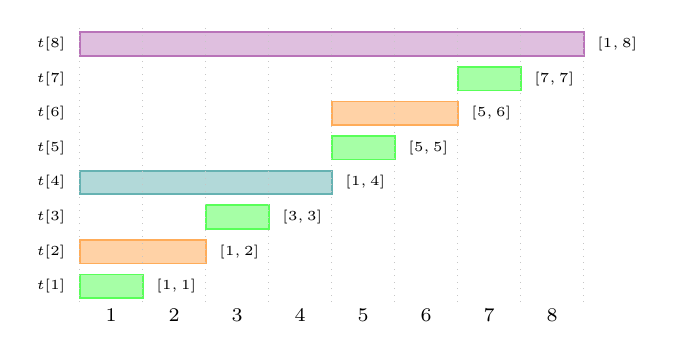
\begin{tikzpicture}
    \def\w{0.80}  % latime per pozitie (cm)
    \def\rh{0.30} % inaltimea unui bar (aceeasi pentru toti)
    \def\s{0.44}  % pas vertical intre baruri (\rh + gap)
    % Baruri orizontale — fiecare t[i] pe propriul rand (de jos in sus)
    % Lungimea = lsb(i) * \w;  pozitia x = (i - lsb(i)) * \w
    % t[1]: [1,1] lsb=1, rand 0 — verde
    \filldraw[fill=green!35,  draw=green!65,  line width=0.6pt]
      (0,      0*\s) rectangle (1*\w, 0*\s+\rh);
    % t[2]: [1,2] lsb=2, rand 1 — portocaliu
    \filldraw[fill=orange!35, draw=orange!65, line width=0.6pt]
      (0,      1*\s) rectangle (2*\w, 1*\s+\rh);
    % t[3]: [3,3] lsb=1, rand 2 — verde
    \filldraw[fill=green!35,  draw=green!65,  line width=0.6pt]
      (2*\w,   2*\s) rectangle (3*\w, 2*\s+\rh);
    % t[4]: [1,4] lsb=4, rand 3 — teal
    \filldraw[fill=teal!30,   draw=teal!60,   line width=0.6pt]
      (0,      3*\s) rectangle (4*\w, 3*\s+\rh);
    % t[5]: [5,5] lsb=1, rand 4 — verde
    \filldraw[fill=green!35,  draw=green!65,  line width=0.6pt]
      (4*\w,   4*\s) rectangle (5*\w, 4*\s+\rh);
    % t[6]: [5,6] lsb=2, rand 5 — portocaliu
    \filldraw[fill=orange!35, draw=orange!65, line width=0.6pt]
      (4*\w,   5*\s) rectangle (6*\w, 5*\s+\rh);
    % t[7]: [7,7] lsb=1, rand 6 — verde
    \filldraw[fill=green!35,  draw=green!65,  line width=0.6pt]
      (6*\w,   6*\s) rectangle (7*\w, 6*\s+\rh);
    % t[8]: [1,8] lsb=8, rand 7 — violet
    \filldraw[fill=violet!25, draw=violet!55, line width=0.6pt]
      (0,      7*\s) rectangle (8*\w, 7*\s+\rh);
    % Etichete stanga
    \node[font=\tiny, anchor=east] at (-0.06, 0*\s+0.5*\rh) {$t[1]$};
    \node[font=\tiny, anchor=east] at (-0.06, 1*\s+0.5*\rh) {$t[2]$};
    \node[font=\tiny, anchor=east] at (-0.06, 2*\s+0.5*\rh) {$t[3]$};
    \node[font=\tiny, anchor=east] at (-0.06, 3*\s+0.5*\rh) {$t[4]$};
    \node[font=\tiny, anchor=east] at (-0.06, 4*\s+0.5*\rh) {$t[5]$};
    \node[font=\tiny, anchor=east] at (-0.06, 5*\s+0.5*\rh) {$t[6]$};
    \node[font=\tiny, anchor=east] at (-0.06, 6*\s+0.5*\rh) {$t[7]$};
    \node[font=\tiny, anchor=east] at (-0.06, 7*\s+0.5*\rh) {$t[8]$};
    % Etichete dreapta — intervalul acoperit
    \node[font=\tiny, anchor=west] at (1*\w+0.05, 0*\s+0.5*\rh) {$[1,1]$};
    \node[font=\tiny, anchor=west] at (2*\w+0.05, 1*\s+0.5*\rh) {$[1,2]$};
    \node[font=\tiny, anchor=west] at (3*\w+0.05, 2*\s+0.5*\rh) {$[3,3]$};
    \node[font=\tiny, anchor=west] at (4*\w+0.05, 3*\s+0.5*\rh) {$[1,4]$};
    \node[font=\tiny, anchor=west] at (5*\w+0.05, 4*\s+0.5*\rh) {$[5,5]$};
    \node[font=\tiny, anchor=west] at (6*\w+0.05, 5*\s+0.5*\rh) {$[5,6]$};
    \node[font=\tiny, anchor=west] at (7*\w+0.05, 6*\s+0.5*\rh) {$[7,7]$};
    \node[font=\tiny, anchor=west] at (8*\w+0.05, 7*\s+0.5*\rh) {$[1,8]$};
    % Linii verticale de referinta
    \foreach \i in {0,...,8} {
      \draw[dotted, gray!45, line width=0.35pt]
        (\i*\w, -0.05) -- (\i*\w, 7*\s+\rh+0.05);
    }
    % Indexuri la baza
    \foreach \i in {1,...,8} {
      \node[font=\scriptsize] at (\i*\w-0.5*\w, -0.22) {\i};
    }
  \end{tikzpicture}
  \end{center}
  \vspace{-4pt}
  {\footnotesize
  \textcolor{green!60!black}{$\blacksquare$}~lsb$=1$\enspace
  \textcolor{orange!70!black}{$\blacksquare$}~lsb$=2$\enspace
  \textcolor{teal!70!black}{$\blacksquare$}~lsb$=4$\enspace
  \textcolor{violet!70!black}{$\blacksquare$}~lsb$=8$\quad
  Lungimea barei $=$ numărul de elemente acoperite.}
\end{frame}

\begin{frame}{Query \textemdash{} Prefix sum $[1, i]$}
  \textbf{Idee:} adunăm $t[i]$, sărim la $i - \text{lsb}(i)$, repetăm până la 0.
  \begin{block}{Traseu pentru \texttt{get(7)}}
    \begin{itemize}\itemsep0pt
      \item $i=7$: $t[7]=a[7]$; $i \leftarrow 7-1 = 6$
      \item $i=6$: $t[6]=a[5]{+}a[6]$; $i \leftarrow 6-2 = 4$
      \item $i=4$: $t[4]=a[1]{+}{\cdots}{+}a[4]$; $i \leftarrow 4-4 = 0$ \textemdash{} stop
    \end{itemize}
    Suma returnată: $a[1]+\cdots+a[7]$ \checkmark
  \end{block}
  \smallskip
  \textbf{Complexitate:} $O(\log n)$ \textemdash{} la fiecare pas se elimină un bit setat.

  Suma pe interval $[l, r]$: \texttt{get(r) - get(l-1)}.
\end{frame}

\begin{frame}{Update \textemdash{} Point add la poziția $i$}
  \textbf{Idee:} actualizăm $t[i]$, sărim la $i + \text{lsb}(i)$, repetăm până depășim $n$.
  \begin{block}{Traseu pentru \texttt{add(3, x)}}
    \begin{itemize}\itemsep0pt
      \item $i=3$: $t[3]\ {+}{=}\ x$; $i \leftarrow 3+1 = 4$
      \item $i=4$: $t[4]\ {+}{=}\ x$; $i \leftarrow 4+4 = 8$
      \item $i=8$: $t[8]\ {+}{=}\ x$; $i \leftarrow 8+8 = 16 > n$ \textemdash{} stop
    \end{itemize}
  \end{block}
  \smallskip
  Actualizăm exact pozițiile al căror interval conține indexul 3:
  $t[3]$ (acoperă $[3,3]$), $t[4]$ (acoperă $[1,4]$), $t[8]$ (acoperă $[1,8]$).

  \textbf{Complexitate:} $O(\log n)$ \textemdash{} la fiecare pas se adaugă un bit.
\end{frame}

\begin{frame}[fragile]{Implementare AIB Clasic}
  \begin{lstlisting}
const int nmax = 100005;
long long t[nmax];
int n;

void add(int i, long long x) {
    for (; i <= n; i += i & -i) {
        t[i] += x;
    }
}

long long get(int i) {
    long long s = 0;
    for (; i > 0; i -= i & -i) {
        s += t[i];
    }
    return s;
}

long long get(int l, int r) {
    return get(r) - get(l - 1);
}
  \end{lstlisting}
\end{frame}

% ================================================================
\section{Range add, point query}

\begin{frame}{Range add, point query \textemdash{} Idee}
  \begin{block}{Problemă}
    \begin{itemize}\itemsep0pt
      \item \textbf{Range add:} adaugă $x$ la toate $a_i$ cu $l \leq i \leq r$
      \item \textbf{Point query:} care e valoarea curentă a lui $a_i$?
    \end{itemize}
  \end{block}
  \smallskip
  \textbf{Transformare cu șir de diferențe:} fie $d[i] = a[i] - a[i-1]$. Atunci:
  \[
    a[i] = \sum_{j=1}^{i} d[j] \quad \Rightarrow \quad
    \text{point query} = \text{prefix sum pe } d
  \]
  \textbf{Operații pe $d$:}
  \begin{itemize}\itemsep0pt
    \item Range add $[l,r]$ cu $x$: $d[l] {+}{=} x$, $d[r{+}1] {-}{=} x$ \textemdash{} 2 actualizări punct
    \item Point query $a[i]$: prefix sum $d[1..i]$ cu \texttt{get(i)}
  \end{itemize}
  \smallskip
  Menținem un \textbf{AIB pe șirul de diferențe $d$}.
  Ambele operații: $O(\log n)$.
\end{frame}

\begin{frame}[fragile]{Range add, point query \textemdash{} Implementare}
  \begin{lstlisting}
const int nmax = 100005;
long long d[nmax]; // AIB pe sirul de diferente
int n;

void range_add(int l, int r, long long x) {
    for (int i = l; i <= n; i += i & -i) {
        d[i] += x;
    }
    for (int i = r + 1; i <= n; i += i & -i) {
        d[i] -= x;
    }
}

long long point_get(int i) {
    long long s = 0;
    for (; i > 0; i -= i & -i) {
        s += d[i];
    }
    return s;
}
  \end{lstlisting}
\end{frame}

% ================================================================
\section{Range add, range sum}

\begin{frame}{Range add, range sum \textemdash{} De ce un singur AIB nu ajunge}
  Știm deja: range add + \textbf{point query} $\rightarrow$ AIB pe șirul de diferențe $d$.

  $a[i] = \texttt{d.get}(i)$. Dar \textbf{range sum} $[l, r]$?
  \[
    P(i) = \sum_{j=1}^{i} a[j]
         = \sum_{j=1}^{i} \sum_{k=1}^{j} d[k]
         = \sum_{k=1}^{i} d[k]\cdot(i - k + 1)
  \]
  Rezultatul depinde atât de $i$ cât și de \emph{care} $d[k]$ sunt nenuli
  \textemdash{} nu putem calcula $P(i)$ dintr-o singură interogare pe AIB.

  \smallskip
  \begin{alertblock}{Soluție}
    Scriem $P(i)$ ca diferența a două prefix sums, fiecare menținut într-un AIB:
    \[
      P(i) = \underbrace{B_1\text{.get}(i)}_{\text{coef. lui }i} \cdot\, i
           \ -\ \underbrace{B_2\text{.get}(i)}_{\text{corecție constantă}}
    \]
    Actualizăm $B_1$ și $B_2$ în $O(\log n)$ la fiecare range add.
  \end{alertblock}
\end{frame}

\begin{frame}{Range add, range sum \textemdash{} Derivarea lui $B_1$ și $B_2$}
  \textbf{Ce se întâmplă cu $P(i)$ după \texttt{range\_add}$(l, r, x)$?}

  \begin{center}
  \begin{tabular}{lll}
    \toprule
    $i < l$ & $l \leq i \leq r$ & $i > r$ \\
    \midrule
    $\Delta P = 0$ & $\Delta P = x(i{-}l{+}1) = \mathbf{x}\cdot i - \mathbf{x(l{-}1)}$
                   & $\Delta P = x(r{-}l{+}1)$ (constant) \\
    \bottomrule
  \end{tabular}
  \end{center}
  \smallskip
  Dacă actualizăm $B_1$, $B_2$ astfel:
  \[
    B_1\text{.add}(l,\,x),\quad B_1\text{.add}(r{+}1,\,-x)
    \qquad
    B_2\text{.add}(l,\,x(l{-}1)),\quad B_2\text{.add}(r{+}1,\,-x\cdot r)
  \]
  atunci $P(i) = B_1\text{.get}(i)\cdot i - B_2\text{.get}(i)$:
  \begin{center}
  {\footnotesize
  \begin{tabular}{l|cc|l}
    & $B_1\text{.get}(i)$ & $B_2\text{.get}(i)$ & $B_1\cdot i - B_2$ \\
    \hline
    $i < l$       & $0$        & $0$           & $0$ \checkmark \\
    $l\leq i\leq r$ & $x$      & $x(l{-}1)$   & $xi - x(l{-}1) = x(i{-}l{+}1)$ \checkmark \\
    $i > r$       & $0$        & $x(l{-}1{-}r)$ & $-x(l{-}1{-}r) = x(r{-}l{+}1)$ \checkmark \\
  \end{tabular}}
  \end{center}
  \smallskip
  \textbf{Range sum:} $\text{sum}(l,r) = P(r) - P(l{-}1)$.
\end{frame}

\begin{frame}[fragile]{Range add, range sum \textemdash{} Implementare}
  \begin{lstlisting}
// add_aib / get_aib: aceleasi ca add/get clasic, cu AIB ca parametru
long long b1[nmax], b2[nmax];
int n;

void range_add(int l, int r, long long x) {
    add_aib(b1, l, x);       add_aib(b1, r + 1, -x);
    add_aib(b2, l, x*(l-1)); add_aib(b2, r + 1, -x*r);
}

long long prefix_sum(int i) {
    return get_aib(b1, i) * i - get_aib(b2, i);
}

long long range_sum(int l, int r) {
    return prefix_sum(r) - prefix_sum(l - 1);
}
  \end{lstlisting}
\end{frame}

% ================================================================
\section{Prefix minimum}

\begin{frame}{Prefix minimum \textemdash{} Idee și limitări}
  \begin{block}{Problemă}
    Dat un șir $a$. Operații:
    \begin{itemize}\itemsep0pt
      \item \textbf{Update:} setează $a[i] = x$ (valoare mai mică decât cea curentă)
      \item \textbf{Prefix min:} calculează $\min(a[1], \ldots, a[i])$
    \end{itemize}
  \end{block}
  \smallskip
  Implementare aproape identică cu AIB-ul clasic, dar cu $\min$ în loc de $+$:
  \begin{itemize}\itemsep0pt
    \item $t[i]$ stochează $\min$ pe intervalul $[i-\text{lsb}(i)+1, i]$
    \item Query: parcurgem ca la sum, dar luăm minimul
    \item Update: actualizăm $t[i] = \min(t[i], x)$ și sărim înainte
  \end{itemize}
  \smallskip
  \begin{alertblock}{Limitări față de AIB cu sumă}
    \begin{itemize}\itemsep0pt
      \item \textbf{Doar prefix} $[1, i]$, \textbf{nu range} $[l, r]$
        \textemdash{} $\min$ nu e invertibil
      \item Update-urile trebuie să fie \textbf{monoton descrescătoare}
        ($x \leq a[i]$ curent)
    \end{itemize}
  \end{alertblock}
\end{frame}

\begin{frame}[fragile]{Prefix minimum \textemdash{} Implementare}
  \begin{lstlisting}
const int nmax = 100005;
const long long INF = 1e18;
long long t[nmax];
int n;

// Initializare: t[i] = INF pentru toti i

void update(int i, long long x) {
    for (; i <= n; i += i & -i) {
        t[i] = min(t[i], x);
    }
}

long long prefix_min(int i) {
    long long res = INF;
    for (; i > 0; i -= i & -i) {
        res = min(res, t[i]);
    }
    return res;
}
  \end{lstlisting}
\end{frame}

% ================================================================
\section{AIB 2D}

\begin{frame}{AIB 2D \textemdash{} Generalizare}
  \begin{block}{Problemă}
    Matrice $n \times m$. Operații:
    \begin{itemize}\itemsep0pt
      \item \textbf{Point add:} adaugă $x$ la $a[i][j]$
      \item \textbf{Prefix 2D sum:} $\sum_{r \leq i,\, c \leq j} a[r][c]$
    \end{itemize}
  \end{block}
  \smallskip
  \textbf{Idee:} aplicăm același salt cu $\text{lsb}$ pe \textbf{ambele dimensiuni}.

  $t[i][j]$ stochează suma pe submatricea
  $[i{-}\text{lsb}(i){+}1, i] \times [j{-}\text{lsb}(j){+}1, j]$.
  \smallskip
  Complexitate: $O(\log n \cdot \log m)$ per operație.
  \smallskip
  \textbf{Suma pe submatrice} $[r_1,c_1] \times [r_2,c_2]$
  prin incluziune-excludere:
  \[
    \texttt{get}(r_2,c_2) - \texttt{get}(r_2,c_1{-}1)
    - \texttt{get}(r_1{-}1,c_2) + \texttt{get}(r_1{-}1,c_1{-}1)
  \]
\end{frame}

\begin{frame}[fragile]{AIB 2D \textemdash{} Implementare}
  \begin{lstlisting}
const int nmax = 1005;
long long t[nmax][nmax];
int n, m;

void add(int i, int j, long long x) {
    for (; i <= n; i += i & -i) {
        for (int y = j; y <= m; y += y & -y) { t[i][y] += x; }
    }
}

long long get(int i, int j) {
    long long s = 0;
    for (; i > 0; i -= i & -i) {
        for (int y = j; y > 0; y -= y & -y) { s += t[i][y]; }
    }
    return s;
}

long long get(int r1, int c1, int r2, int c2) {
    return get(r2,c2) - get(r2,c1-1)
         - get(r1-1,c2) + get(r1-1,c1-1);
}
  \end{lstlisting}
\end{frame}

% ================================================================
\section{Recapitulare}

\begin{frame}{Recapitulare}
  \begin{center}
  {\footnotesize
  \begin{tabular}{llll}
    \toprule
    Variantă & Update & Query & Condiție \\
    \midrule
    Point add, range sum & $O(\log n)$ & $O(\log n)$ & \textemdash{} \\
    Range add, point query & $O(\log n)$ & $O(\log n)$ & \textemdash{} \\
    Range add, range sum & $O(\log n)$ & $O(\log n)$ & \textemdash{} \\
    Prefix minimum & $O(\log n)$ & $O(\log n)$ & update monoton $\downarrow$ \\
    AIB 2D & $O(\log^2 n)$ & $O(\log^2 n)$ & \textemdash{} \\
    \bottomrule
  \end{tabular}}
  \end{center}
  \smallskip
  \textbf{AIB vs. Segment Tree:}
  \begin{itemize}\itemsep0pt
    \item[+] Implementare mai scurtă, constantă mai mică, memorie exactă $O(n)$
    \item[$-$] Funcționează \textbf{doar cu operații inversabile} (sumă, XOR)
    \item[$-$] Range min/max, lazy propagation $\rightarrow$ Segment Tree
  \end{itemize}
\end{frame}

\begin{frame}{Probleme de antrenament}
  \begin{enumerate}
    \item \href{https://cses.fi/problemset/task/1648}{\textbf{Point Add Range Sum}}
          \textcolor{gray}{(CSES \#1648 \textemdash{} AIB clasic)}
    \item \href{https://cses.fi/problemset/task/1651}{\textbf{Range Update Queries}}
          \textcolor{gray}{(CSES \#1651 \textemdash{} range add, point query)}
    \item \href{https://cses.fi/problemset/task/1652}{\textbf{Forest Queries II}}
          \textcolor{gray}{(CSES \#1739 \textemdash{} AIB 2D)}
    \item \href{https://cses.fi/problemset/task/1145}{\textbf{Increasing Subsequence}}
          \textcolor{gray}{(CSES \#1145 \textemdash{} SCLM cu AIB prefix min)}
    \item \href{https://infoarena.ro/problema/aib}{\textbf{AIB}}
          \textcolor{gray}{(infoarena \textemdash{} problemă clasică)}
    \item \href{https://kilonova.ro/problems/2669}{\textbf{perm}}
          \textcolor{gray}{(Kilonova \#2669 \textemdash{} ONI 2024 Baraj Seniori)}
  \end{enumerate}
\end{frame}

\begin{frame}{Resurse}
  \begin{enumerate}
    \item \href{https://cp-algorithms.com/data_structures/fenwick.html}{\textbf{CP-Algorithms}}
          \textemdash{} Fenwick Tree (EN, foarte complet cu dovezi)
    \item \href{https://usaco.guide/gold/PURS}{\textbf{USACO Guide}}
          \textemdash{} Point Update Range Sum (Gold)
    \item \href{https://brilliant.org/wiki/fenwick-tree/}{\textbf{Brilliant}}
          \textemdash{} Fenwick Tree (EN, accesibil)
    \item \href{https://en.algorithmica.org/hpc/data-structures/segment-trees/\#fenwick-trees}{\textbf{Algorithmica}}
          \textemdash{} AIB vs. Segment Tree cu benchmark-uri
  \end{enumerate}
\end{frame}

\end{document}
